% Options for packages loaded elsewhere
\PassOptionsToPackage{unicode}{hyperref}
\PassOptionsToPackage{hyphens}{url}
%
\documentclass[
]{book}
\usepackage{amsmath,amssymb}
\usepackage{lmodern}
\usepackage{iftex}
\ifPDFTeX
  \usepackage[T1]{fontenc}
  \usepackage[utf8]{inputenc}
  \usepackage{textcomp} % provide euro and other symbols
\else % if luatex or xetex
  \usepackage{unicode-math}
  \defaultfontfeatures{Scale=MatchLowercase}
  \defaultfontfeatures[\rmfamily]{Ligatures=TeX,Scale=1}
\fi
% Use upquote if available, for straight quotes in verbatim environments
\IfFileExists{upquote.sty}{\usepackage{upquote}}{}
\IfFileExists{microtype.sty}{% use microtype if available
  \usepackage[]{microtype}
  \UseMicrotypeSet[protrusion]{basicmath} % disable protrusion for tt fonts
}{}
\makeatletter
\@ifundefined{KOMAClassName}{% if non-KOMA class
  \IfFileExists{parskip.sty}{%
    \usepackage{parskip}
  }{% else
    \setlength{\parindent}{0pt}
    \setlength{\parskip}{6pt plus 2pt minus 1pt}}
}{% if KOMA class
  \KOMAoptions{parskip=half}}
\makeatother
\usepackage{xcolor}
\IfFileExists{xurl.sty}{\usepackage{xurl}}{} % add URL line breaks if available
\IfFileExists{bookmark.sty}{\usepackage{bookmark}}{\usepackage{hyperref}}
\hypersetup{
  pdftitle={Various exercises on programming in R},
  pdfauthor={Bram Kuijper},
  hidelinks,
  pdfcreator={LaTeX via pandoc}}
\urlstyle{same} % disable monospaced font for URLs
\usepackage{color}
\usepackage{fancyvrb}
\newcommand{\VerbBar}{|}
\newcommand{\VERB}{\Verb[commandchars=\\\{\}]}
\DefineVerbatimEnvironment{Highlighting}{Verbatim}{commandchars=\\\{\}}
% Add ',fontsize=\small' for more characters per line
\usepackage{framed}
\definecolor{shadecolor}{RGB}{248,248,248}
\newenvironment{Shaded}{\begin{snugshade}}{\end{snugshade}}
\newcommand{\AlertTok}[1]{\textcolor[rgb]{0.94,0.16,0.16}{#1}}
\newcommand{\AnnotationTok}[1]{\textcolor[rgb]{0.56,0.35,0.01}{\textbf{\textit{#1}}}}
\newcommand{\AttributeTok}[1]{\textcolor[rgb]{0.77,0.63,0.00}{#1}}
\newcommand{\BaseNTok}[1]{\textcolor[rgb]{0.00,0.00,0.81}{#1}}
\newcommand{\BuiltInTok}[1]{#1}
\newcommand{\CharTok}[1]{\textcolor[rgb]{0.31,0.60,0.02}{#1}}
\newcommand{\CommentTok}[1]{\textcolor[rgb]{0.56,0.35,0.01}{\textit{#1}}}
\newcommand{\CommentVarTok}[1]{\textcolor[rgb]{0.56,0.35,0.01}{\textbf{\textit{#1}}}}
\newcommand{\ConstantTok}[1]{\textcolor[rgb]{0.00,0.00,0.00}{#1}}
\newcommand{\ControlFlowTok}[1]{\textcolor[rgb]{0.13,0.29,0.53}{\textbf{#1}}}
\newcommand{\DataTypeTok}[1]{\textcolor[rgb]{0.13,0.29,0.53}{#1}}
\newcommand{\DecValTok}[1]{\textcolor[rgb]{0.00,0.00,0.81}{#1}}
\newcommand{\DocumentationTok}[1]{\textcolor[rgb]{0.56,0.35,0.01}{\textbf{\textit{#1}}}}
\newcommand{\ErrorTok}[1]{\textcolor[rgb]{0.64,0.00,0.00}{\textbf{#1}}}
\newcommand{\ExtensionTok}[1]{#1}
\newcommand{\FloatTok}[1]{\textcolor[rgb]{0.00,0.00,0.81}{#1}}
\newcommand{\FunctionTok}[1]{\textcolor[rgb]{0.00,0.00,0.00}{#1}}
\newcommand{\ImportTok}[1]{#1}
\newcommand{\InformationTok}[1]{\textcolor[rgb]{0.56,0.35,0.01}{\textbf{\textit{#1}}}}
\newcommand{\KeywordTok}[1]{\textcolor[rgb]{0.13,0.29,0.53}{\textbf{#1}}}
\newcommand{\NormalTok}[1]{#1}
\newcommand{\OperatorTok}[1]{\textcolor[rgb]{0.81,0.36,0.00}{\textbf{#1}}}
\newcommand{\OtherTok}[1]{\textcolor[rgb]{0.56,0.35,0.01}{#1}}
\newcommand{\PreprocessorTok}[1]{\textcolor[rgb]{0.56,0.35,0.01}{\textit{#1}}}
\newcommand{\RegionMarkerTok}[1]{#1}
\newcommand{\SpecialCharTok}[1]{\textcolor[rgb]{0.00,0.00,0.00}{#1}}
\newcommand{\SpecialStringTok}[1]{\textcolor[rgb]{0.31,0.60,0.02}{#1}}
\newcommand{\StringTok}[1]{\textcolor[rgb]{0.31,0.60,0.02}{#1}}
\newcommand{\VariableTok}[1]{\textcolor[rgb]{0.00,0.00,0.00}{#1}}
\newcommand{\VerbatimStringTok}[1]{\textcolor[rgb]{0.31,0.60,0.02}{#1}}
\newcommand{\WarningTok}[1]{\textcolor[rgb]{0.56,0.35,0.01}{\textbf{\textit{#1}}}}
\usepackage{longtable,booktabs,array}
\usepackage{calc} % for calculating minipage widths
% Correct order of tables after \paragraph or \subparagraph
\usepackage{etoolbox}
\makeatletter
\patchcmd\longtable{\par}{\if@noskipsec\mbox{}\fi\par}{}{}
\makeatother
% Allow footnotes in longtable head/foot
\IfFileExists{footnotehyper.sty}{\usepackage{footnotehyper}}{\usepackage{footnote}}
\makesavenoteenv{longtable}
\usepackage{graphicx}
\makeatletter
\def\maxwidth{\ifdim\Gin@nat@width>\linewidth\linewidth\else\Gin@nat@width\fi}
\def\maxheight{\ifdim\Gin@nat@height>\textheight\textheight\else\Gin@nat@height\fi}
\makeatother
% Scale images if necessary, so that they will not overflow the page
% margins by default, and it is still possible to overwrite the defaults
% using explicit options in \includegraphics[width, height, ...]{}
\setkeys{Gin}{width=\maxwidth,height=\maxheight,keepaspectratio}
% Set default figure placement to htbp
\makeatletter
\def\fps@figure{htbp}
\makeatother
\setlength{\emergencystretch}{3em} % prevent overfull lines
\providecommand{\tightlist}{%
  \setlength{\itemsep}{0pt}\setlength{\parskip}{0pt}}
\setcounter{secnumdepth}{5}
\usepackage{booktabs}
\usepackage{amsthm}
\makeatletter
\def\thm@space@setup{%
  \thm@preskip=8pt plus 2pt minus 4pt
  \thm@postskip=\thm@preskip
}
\makeatother
\ifLuaTeX
  \usepackage{selnolig}  % disable illegal ligatures
\fi
\usepackage[]{natbib}
\bibliographystyle{apalike}

\title{Various exercises on programming in R}
\author{Bram Kuijper}
\date{2022-01-28}

\begin{document}
\maketitle

{
\setcounter{tocdepth}{1}
\tableofcontents
}
\hypertarget{introduction}{%
\chapter{Introduction}\label{introduction}}

Here a small selection of problems to get some practical exposure to R programming. Some of these exercises may be quite relevant to one's work, other may be less so. However, relevance to one's work is not a really good criterion here; we simply want to practice problem solving.

\hypertarget{prior-knowledge-about-r}{%
\section{Prior knowledge about R}\label{prior-knowledge-about-r}}

This set of exercises assumes you already have a reasonable understanding of the R basics. Here a bunch of different sources that provide an overview of the R basics:

\begin{itemize}
\tightlist
\item
  Chapters 1-8 of the book \emph{The Book of R} \citep{Davies2016}, which is available in UExeter's library \href{https://encore.exeter.ac.uk/iii/encore/record/C__Rb3554370}{here}
\item
  \href{https://cran.r-project.org/doc/manuals/r-release/R-intro.html}{An introduction to R} freely available from the R website.
\item
  Chapter 2 of the book \emph{The R Book} \citep{Crawley2013}, which is available in UExeter's library \href{https://encore.exeter.ac.uk/iii/encore/record/C__Rb3361719}{here}
\item
  Chapter 1-7 of the book \emph{The Art of R Programming} \citep{Matloff2011}, which is available in UExeter's library \href{https://encore.exeter.ac.uk/iii/encore/record/C__Rb3509192}{here}
\end{itemize}

One should not search for pdfs of these books online.

\hypertarget{finding-help}{%
\subsection{Finding help}\label{finding-help}}

Next to googling everything you don't understand, you can also find help using the \href{https://stat.ethz.ch/R-manual/R-devel/library/utils/html/Question.html}{\texttt{?}} command in R's built-in help pages. For example, you can use the \texttt{?} preceding a certain function or variable. For example, in case we want more information about R's \href{https://stat.ethz.ch/R-manual/R-devel/library/utils/html/str.html}{\texttt{str()}} function, we simply type

\begin{Shaded}
\begin{Highlighting}[]
\NormalTok{?str}
\end{Highlighting}
\end{Shaded}

Obviously, next to R's built-in help pages, search engines are your friend when you hunt for examples.

\textbf{Pro-tip: use quotation marks \texttt{""} when consulting help for operators and weird characters} For operators and things with weird characters, using the \texttt{?} help function may not bring you very far. For example, let's say you are interested in finding out about R's \href{https://stat.ethz.ch/R-manual/R-devel/library/base/html/match.html}{\texttt{\%in\%}} matching operator:

\begin{Shaded}
\begin{Highlighting}[]
\NormalTok{?}\SpecialCharTok{\%in\%}
\DocumentationTok{\#\# Error: \textless{}text\textgreater{}:1:2: unexpected SPECIAL}
\DocumentationTok{\#\# 1: ?\%in\%}
\DocumentationTok{\#\#      \^{}}
\end{Highlighting}
\end{Shaded}

Clearly, R chokes on the \texttt{\%} character. What now? Easy, just use quotes:

\begin{Shaded}
\begin{Highlighting}[]
\NormalTok{?}\StringTok{"\%in\%"}
\end{Highlighting}
\end{Shaded}

\hypertarget{different-types-of-variables}{%
\subsection{Different types of variables}\label{different-types-of-variables}}

You know about variables and different types of data such as \texttt{character}, \texttt{logical}. Also,you know about different data structures such as \href{https://stat.ethz.ch/R-manual/R-devel/library/base/html/c.html}{\texttt{c()}} (vectors), \href{https://stat.ethz.ch/R-manual/R-devel/library/base/html/data.frame.html}{\texttt{data.frame}}s and \href{https://stat.ethz.ch/R-manual/R-devel/library/base/html/list.html}{\texttt{list}}s. Finally, you know that the \href{https://stat.ethz.ch/R-manual/R-devel/library/base/html/typeof.html}{\texttt{typeof()}} function can be used to find out what data is contained in a data type. Similarly, also the \href{https://stat.ethz.ch/R-manual/R-devel/library/utils/html/str.html}{\texttt{str()}} helps you to find out more about the structure of a data type. Please see \href{https://swcarpentry.github.io/r-novice-inflammation/13-supp-data-structures/}{here} for a fantastic overview of the different data types and key data structures.

\hypertarget{operators}{%
\subsection{Operators}\label{operators}}

Please click the corresponding links if you do not know about \href{https://stat.ethz.ch/R-manual/R-devel/library/base/html/Arithmetic.html}{arithmetic operators} such as \texttt{*} (multiplication), \texttt{\^{}} (power), \texttt{\%\%} (modulo). The same goes for \href{https://stat.ethz.ch/R-manual/R-devel/library/base/html/Logic.html}{logical operators} such as \texttt{\textbar{}\textbar{}} (which is the \texttt{OR} operator) and \href{https://stat.ethz.ch/R-manual/R-devel/library/base/html/Comparison.html}{relational operators} such as \texttt{\textgreater{}=} (which is the greater-than-or-equal-operator). See \href{https://bookdown.org/swen/R_for_Everyone/L03.html\#r-as-a-calculator}{Chapter 4} for a brief overview.

\hypertarget{control-flow}{%
\subsection{Control flow}\label{control-flow}}

Things like \texttt{if}-\texttt{else} statements and \href{https://stat.ethz.ch/R-manual/R-devel/library/base/html/ifelse.html}{\texttt{ifelse()}} functions should be understood. Read the freely available \href{https://adv-r.hadley.nz/control-flow.html}{Chapter 5} from \citep{Wickham2019} for more information, or chapter 7 of \citep{Matloff2011}

\hypertarget{sizes-of-things}{%
\subsection{Sizes of things}\label{sizes-of-things}}

To use loops, knowing the sizes of things in R is important. Hence, you know how to obtain the \href{https://stat.ethz.ch/R-manual/R-devel/library/base/html/length.html}{\texttt{length()}} of a vector, or the number of characters in a string of text using \href{https://stat.ethz.ch/R-manual/R-devel/library/base/html/nchar.html}{\texttt{nchar()}}. You also know how to obtain the number of rows and columns of a \texttt{data.frame}, using \href{https://stat.ethz.ch/R-manual/R-devel/library/base/html/nrow.html}{\texttt{nrow()}}, \href{https://stat.ethz.ch/R-manual/R-devel/library/base/html/ncol.html}{\texttt{ncol()}} or its dimensions using \href{https://stat.ethz.ch/R-manual/R-devel/library/base/html/dim.html}{\texttt{dim()}}.

\hypertarget{selecting-subsets-of-your-data}{%
\section{Selecting subsets of your data}\label{selecting-subsets-of-your-data}}

You know the difference between \texttt{iris{[},1{]}}, \texttt{iris{[}1,{]}} and \texttt{iris{[}1,1{]}}? See \href{https://adv-r.hadley.nz/subsetting.html}{Chapter 4} for a great overview of how to subset your data in different ways.

\hypertarget{loop-structures}{%
\subsection{Loop structures}\label{loop-structures}}

You will need to have read about \texttt{for}-loops and potentially also about \href{https://stat.ethz.ch/R-manual/R-devel/library/base/html/switch.html}{\texttt{switch()}} statements. Check out chapter 7 of \citep{Matloff2011}, chapter 21 of \citep{Wickham2017} (available online) or check online for videos on these topics. For example, using the search terms \texttt{for\ loops\ in\ R} provides a bunch of great videos.

\hypertarget{some-additional-coding-tips}{%
\section{Some additional coding tips:}\label{some-additional-coding-tips}}

\hypertarget{dont-ignore-the-links-and-hints}{%
\subsection{Don't ignore the links and hints}\label{dont-ignore-the-links-and-hints}}

Sometimes there are hints provided in the exercises, for example:
``You can do this by using the \href{https://stat.ethz.ch/R-manual/R-patched/library/base/html/paste.html}{\texttt{paste()}} function'', which involves
you reading the documentation on this function and trying
some of the provided examples in the documentation. I typically provide hyperlinks to the documentation, which is why the \href{https://stat.ethz.ch/R-manual/R-patched/library/base/html/paste.html}{\texttt{paste()}} function here is given in blue. Click on them and read them. Please do.

\hypertarget{try-out-examples-for-yourself}{%
\subsection{Try out examples for yourself}\label{try-out-examples-for-yourself}}

When reading a book, try the code examples and snippets for yourself, by typing them out (don't copy-paste them, unless it is a massive amount of code). Only by typing out do you see what's going on and will you start to memorize the different coding constructs. Moreover, you are bound to make occasional mistakes! And mistakes are good, as the earlier you learn how to hunt for coding errors and solving mistakes the better.

\hypertarget{search-enginges-are-your-friend}{%
\subsection{Search enginges are your friend}\label{search-enginges-are-your-friend}}

Search engines are your friend. If some function or construct is used that is new to one, google what it is about. Say, one encounters the statement

\begin{Shaded}
\begin{Highlighting}[]
\NormalTok{means }\OtherTok{\textless{}{-}} \FunctionTok{apply}\NormalTok{(}\AttributeTok{X=}\NormalTok{cars,}\AttributeTok{MARGIN=}\DecValTok{2}\NormalTok{,}\AttributeTok{FUN=}\NormalTok{mean)}
\end{Highlighting}
\end{Shaded}

and one does not know what the \href{https://stat.ethz.ch/R-manual/R-devel/library/base/html/apply.html}{\texttt{apply}} statement is about or what the \texttt{cars} variable is about, I'd immediately search for \texttt{apply\ r} or \texttt{cars\ r}.

\hypertarget{comment-your-code}{%
\subsection{Comment your code}\label{comment-your-code}}

Always try to briefly comment each statement (or group of statements), using \texttt{\#}.

\begin{Shaded}
\begin{Highlighting}[]
\CommentTok{\# select even numbers}
\NormalTok{even\_odd }\OtherTok{\textless{}{-}} \FunctionTok{c}\NormalTok{(}\DecValTok{1}\NormalTok{,}\DecValTok{2}\NormalTok{,}\DecValTok{3}\NormalTok{,}\DecValTok{4}\NormalTok{,}\DecValTok{5}\NormalTok{,}\DecValTok{6}\NormalTok{,}\DecValTok{7}\NormalTok{,}\DecValTok{8}\NormalTok{) }\SpecialCharTok{\%\%} \DecValTok{2} \SpecialCharTok{==} \DecValTok{0}
\end{Highlighting}
\end{Shaded}

\hypertarget{keep-an-error-record}{%
\subsection{Keep an error record}\label{keep-an-error-record}}

Try to keep a record of all the main error messages you encounter, so that you build a record of different error messages and how they have eventually been resolved. This serves as a great lookup tool for recurring errors.

An entry in my error record reads, for example:

\begin{Shaded}
\begin{Highlighting}[]
\FunctionTok{apply}\NormalTok{(}\AttributeTok{X=}\NormalTok{cars,}\AttributeTok{MARGIN=}\DecValTok{2}\NormalTok{,}\AttributeTok{FUN=}\FunctionTok{mean}\NormalTok{())}
\DocumentationTok{\#\# Error in mean.default(): argument "x" is missing, with no default}
\end{Highlighting}
\end{Shaded}

This error occurs because the supplied \texttt{mean()} function used to calculate means of the different columns is provided with parentheses \texttt{()}. However, in order for this function to actually calculate means of each column, you simply need to provide the function name \texttt{mean} without the parentheses, or:

\begin{Shaded}
\begin{Highlighting}[]
\FunctionTok{apply}\NormalTok{(}\AttributeTok{X=}\NormalTok{cars,}\AttributeTok{MARGIN=}\DecValTok{2}\NormalTok{,}\AttributeTok{FUN=}\NormalTok{mean)}
\DocumentationTok{\#\# speed  dist }
\DocumentationTok{\#\# 15.40 42.98}
\end{Highlighting}
\end{Shaded}

\hypertarget{find-out-the-root-of-errors-using-traceback}{%
\subsection{\texorpdfstring{Find out the root of errors using \texttt{traceback()}}{Find out the root of errors using traceback()}}\label{find-out-the-root-of-errors-using-traceback}}

If you stumble upon an error, use R's \href{https://stat.ethz.ch/R-manual/R-devel/library/base/html/traceback.html}{\texttt{traceback()}} function to find the root cause. As \texttt{traceback()} can produce a lot of garbage, it may help to reduce the amount of output, for example by stating \texttt{traceback(max.lines=5)}.

\hypertarget{inspect-values-using-print-or-use-rs-debugger}{%
\subsection{\texorpdfstring{Inspect values using \texttt{print()} or use R's debugger}{Inspect values using print() or use R's debugger}}\label{inspect-values-using-print-or-use-rs-debugger}}

When you have just started to code in R, use as many \href{https://stat.ethz.ch/R-manual/R-patched/library/base/html/print.html}{\texttt{print()}} statements as possible, to obtain information about the state of your program and the values of your variables. When you become more experienced, you can start to inform yourself about R's very handy debugging tools that can do all the variable inspection work for you. Read more about R debugging in the freely available \href{https://adv-r.hadley.nz/debugging.html}{chapter 22} of \citep{Wickham2019}.

\hypertarget{using-loops-to-calculate-sums-and-sums-of-squares}{%
\chapter{Using loops to calculate sums and sums of squares}\label{using-loops-to-calculate-sums-and-sums-of-squares}}

We often use loops to go over series of values and perform operations on them. While more advanced R users typically use techniques such as \href{https://csgillespie.github.io/efficientR/programming.html\#vectorised-code}{vectorization}, or functions such as \href{https://rdrr.io/r/base/lapply.html}{\texttt{lapply()}}, using basic \texttt{for} loops is often the best thing to use when going over a series of values. Here we practice this by performing operations over a simple list of values.

\hypertarget{printEx}{%
\section{Exercise: printing elements from a vector}\label{printEx}}

Here we have the following vector of values:

\begin{Shaded}
\begin{Highlighting}[]
\CommentTok{\# a list of values}
\NormalTok{my.list }\OtherTok{\textless{}{-}} \FunctionTok{c}\NormalTok{(}\DecValTok{5}\NormalTok{,}\DecValTok{10}\NormalTok{,}\DecValTok{19}\NormalTok{,}\DecValTok{22}\NormalTok{,}\DecValTok{3}\NormalTok{,}\DecValTok{40}\NormalTok{,}\DecValTok{48}\NormalTok{)}
\end{Highlighting}
\end{Shaded}

Produce a \texttt{for} loop that uses the \href{https://stat.ethz.ch/R-manual/R-devel/library/base/html/print.html}{\texttt{print()}} function to print each value to the console, resulting in
the following output:

\begin{verbatim}
## [1] 5
## [1] 10
## [1] 19
## [1] 22
## [1] 3
## [1] 40
## [1] 48
\end{verbatim}

\hypertarget{exercise-printing-every-nth-row-from-a-data.frame}{%
\section{\texorpdfstring{Exercise: printing every \(n\)th row from a \texttt{data.frame}}{Exercise: printing every nth row from a data.frame}}\label{exercise-printing-every-nth-row-from-a-data.frame}}

Let us use the built-in \texttt{cars} dataset. Use a \texttt{for} loop to go over the rows of this \texttt{data.frame} and then use the \href{https://stat.ethz.ch/R-manual/R-devel/library/base/html/print.html}{\texttt{print()}} function to print every 10th row, as in

\begin{verbatim}
##   speed dist
## 1     4    2
##    speed dist
## 11    11   28
##    speed dist
## 21    14   36
##    speed dist
## 31    17   50
##    speed dist
## 41    20   52
\end{verbatim}

\hypertarget{sum}{%
\section{Exercise: summing a vector}\label{sum}}

Produce a single \texttt{for} loop to calculate the sum of \texttt{my.list}
in exercise \ref{printEx}. This is chiefly for the sake of
practice, as in reality we would use the \href{https://rdrr.io/r/base/sum.html}{\texttt{sum()}}
function for this. The only output of your script should be:

\begin{verbatim}
## [1] "The sum of the list is 147"
\end{verbatim}

which can be done using the functions \href{https://www.rdocumentation.org/packages/base/versions/3.6.2/topics/print}{\texttt{print()}}
and, in particular, \href{https://www.rdocumentation.org/packages/base/versions/3.6.2/topics/paste}{\texttt{paste()}} which allows you to concatenate strings (pieces of text) and numbers into one sentence.

\hypertarget{sumSq}{%
\section{Sums of squares}\label{sumSq}}

Now copy-paste and modify the code from exercise \ref{sum}
to calculate both the sum
and the sum of squares within one and the same \texttt{for} loop.
Calculating the sum of squares is the same as first squaring each
numbers and then summing these squares, i.e., \(5\times 5 + 10 \times 10 + \cdots + 48 \times 48\).

The program should have no output, other than the
following message at the end:

\begin{verbatim}
## [1] "The sum is 147 and the sum of squares is 4883"
\end{verbatim}

and again, this can be realized using the functions \texttt{print()} and \texttt{paste()}.

\hypertarget{sum-only-if-larger-than-x}{%
\section{\texorpdfstring{Sum only if larger than \(x\)}{Sum only if larger than x}}\label{sum-only-if-larger-than-x}}

Copy-paste the code from exercise \ref{sumSq}
and use an \texttt{if}-statement
to calculate the sum and
the sum of squares for those numbers in the list above
that are greater or equal than \(x=10\). Other numbers
can be ignored. The resulting message should now be:

\begin{verbatim}
## [1] "The sum is 139 and the sum of squares is 4849"
\end{verbatim}

\hypertarget{separate-sums-for-odd-and-even-numbers}{%
\section{Separate sums for odd and even numbers}\label{separate-sums-for-odd-and-even-numbers}}

Copy-paste the code from exercise \ref{sumSq}
and modify it to calculate sums and
sums of squares
for odd and even numbers separately.
Do this using an \texttt{if}-\texttt{else}
statement. The resulting code should print
the following two messages:

\begin{verbatim}
## [1] "Sum of even numbers is 120. Sum of even squares is 4488."
## [1] "Sum of odd numbers is 27. Sum of odd squares is 395."
\end{verbatim}

Note the punctuation in the output above, which was
not there before and requires some changes in the \texttt{paste()}
statement.

\textbf{Hint:} to find out whether a number is odd or even,
use the modulo operator \texttt{a\ \%\%\ b}. This gives the remainder of
the division \texttt{a/b}. For example,

\begin{Shaded}
\begin{Highlighting}[]
\DecValTok{33} \SpecialCharTok{\%\%} \DecValTok{3} 
\DocumentationTok{\#\# [1] 0}
\DecValTok{33} \SpecialCharTok{\%\%} \DecValTok{2} 
\DocumentationTok{\#\# [1] 1}
\DecValTok{33} \SpecialCharTok{\%\%} \DecValTok{5} 
\DocumentationTok{\#\# [1] 3}
\DecValTok{33} \SpecialCharTok{\%\%} \DecValTok{10} 
\DocumentationTok{\#\# [1] 3}
\end{Highlighting}
\end{Shaded}

\hypertarget{produce-a-vector-of-cumulative-values}{%
\section{Produce a vector of cumulative values}\label{produce-a-vector-of-cumulative-values}}

Say, you have a vector of values, called \texttt{a.vec}. From this vector, one can produce another vector, called a cumulative vector, which is often used to develop sampling distributions. The \(i\)th index of such a vector contains the sum of elements from element \(1\) to \(i\). For example, for the following vector

\begin{Shaded}
\begin{Highlighting}[]
\NormalTok{a.vec }\OtherTok{\textless{}{-}} \FunctionTok{c}\NormalTok{(}\DecValTok{5}\NormalTok{,}\DecValTok{9}\NormalTok{,}\DecValTok{1}\NormalTok{,}\DecValTok{3}\NormalTok{,}\DecValTok{12}\NormalTok{,}\DecValTok{8}\NormalTok{,}\DecValTok{50}\NormalTok{,}\DecValTok{82}\NormalTok{,}\DecValTok{1}\NormalTok{,}\DecValTok{9}\NormalTok{,}\DecValTok{2}\NormalTok{,}\DecValTok{7}\NormalTok{)}
\end{Highlighting}
\end{Shaded}

the corresponding cumulative vector should contain the following sequence of values:

\begin{verbatim}
##  [1]   5  14  15  18  30  38  88 170 171 180 182 189
\end{verbatim}

\begin{enumerate}
\def\labelenumi{\arabic{enumi}.}
\tightlist
\item
  Develop code that produces a cumulative vector for the vector \texttt{a.vec} above, where the cumulative vector should be contained in the variable \texttt{cumul.vec}. The variable \texttt{cumul.vec} should be initialized before the start of the \texttt{for}-loop as an \texttt{NA}-filled vector of the same length as \texttt{a.vec}.
\item
  Now, we assign \texttt{a.vec\ \textless{}-\ iris{[},1{]}}. Without any further changes to your code, it should now fill \texttt{cumul.vec} with cumulative values for this new version of \texttt{a.vec}. Output should now be:
\end{enumerate}

\begin{verbatim}
##   [1]   5.1  10.0  14.7  19.3  24.3  29.7  34.3  39.3  43.7  48.6  54.0  58.8
##  [13]  63.6  67.9  73.7  79.4  84.8  89.9  95.6 100.7 106.1 111.2 115.8 120.9
##  [25] 125.7 130.7 135.7 140.9 146.1 150.8 155.6 161.0 166.2 171.7 176.6 181.6
##  [37] 187.1 192.0 196.4 201.5 206.5 211.0 215.4 220.4 225.5 230.3 235.4 240.0
##  [49] 245.3 250.3 257.3 263.7 270.6 276.1 282.6 288.3 294.6 299.5 306.1 311.3
##  [61] 316.3 322.2 328.2 334.3 339.9 346.6 352.2 358.0 364.2 369.8 375.7 381.8
##  [73] 388.1 394.2 400.6 407.2 414.0 420.7 426.7 432.4 437.9 443.4 449.2 455.2
##  [85] 460.6 466.6 473.3 479.6 485.2 490.7 496.2 502.3 508.1 513.1 518.7 524.4
##  [97] 530.1 536.3 541.4 547.1 553.4 559.2 566.3 572.6 579.1 586.7 591.6 598.9
## [109] 605.6 612.8 619.3 625.7 632.5 638.2 644.0 650.4 656.9 664.6 672.3 678.3
## [121] 685.2 690.8 698.5 704.8 711.5 718.7 724.9 731.0 737.4 744.6 752.0 759.9
## [133] 766.3 772.6 778.7 786.4 792.7 799.1 805.1 812.0 818.7 825.6 831.4 838.2
## [145] 844.9 851.6 857.9 864.4 870.6 876.5
\end{verbatim}

\hypertarget{slightly-more-advanced-for-loops}{%
\chapter{Slightly more advanced for loops}\label{slightly-more-advanced-for-loops}}

In this set of exercises we will look at slightly more complicated for loops.

\hypertarget{exercise-a-list-of-random-letters}{%
\section{Exercise: a list of random letters}\label{exercise-a-list-of-random-letters}}

The \texttt{LETTERS}

\hypertarget{exercise-changes-in-state-over-time}{%
\section{Exercise: changes in state over time}\label{exercise-changes-in-state-over-time}}

In many biological models, we model environments that change between two states, \texttt{0} and \texttt{1}. For example, these environments may represent a dry vs a hot environment. Let \(\phi\) reflect the probability that an environment changes from one state to another.

\hypertarget{exercise-select-columns-of-a-data.frame-containing-floating-point-numbers}{%
\section{\texorpdfstring{Exercise: select columns of a \texttt{data.frame} containing floating-point numbers}{Exercise: select columns of a data.frame containing floating-point numbers}}\label{exercise-select-columns-of-a-data.frame-containing-floating-point-numbers}}

Data types like \href{https://stat.ethz.ch/R-manual/R-devel/library/base/html/data.frame.html}{\texttt{data.frames}} and \href{https://tibble.tidyverse.org/}{\texttt{tibbles}} are collections of variables ordered in rows and columns, like a spreadsheet. Take for example the \texttt{Cars93} \texttt{data.frame} from R's \texttt{MASS} package, which we inspect with the \href{https://stat.ethz.ch/R-manual/R-devel/library/utils/html/str.html}{\texttt{str()}} command:

\begin{Shaded}
\begin{Highlighting}[]
\FunctionTok{library}\NormalTok{(}\StringTok{"MASS"}\NormalTok{)}
\FunctionTok{str}\NormalTok{(Cars93)}
\DocumentationTok{\#\# \textquotesingle{}data.frame\textquotesingle{}:    93 obs. of  27 variables:}
\DocumentationTok{\#\#  $ Manufacturer      : Factor w/ 32 levels "Acura","Audi",..: 1 1 2 2 3 4 4 4 4 5 ...}
\DocumentationTok{\#\#  $ Model             : Factor w/ 93 levels "100","190E","240",..: 49 56 9 1 6 24 54 74 73 35 ...}
\DocumentationTok{\#\#  $ Type              : Factor w/ 6 levels "Compact","Large",..: 4 3 1 3 3 3 2 2 3 2 ...}
\DocumentationTok{\#\#  $ Min.Price         : num  12.9 29.2 25.9 30.8 23.7 14.2 19.9 22.6 26.3 33 ...}
\DocumentationTok{\#\#  $ Price             : num  15.9 33.9 29.1 37.7 30 15.7 20.8 23.7 26.3 34.7 ...}
\NormalTok{...}
\end{Highlighting}
\end{Shaded}

Sometimes, we would like to select certain columns from such a \texttt{data.frame}, dependent on a particular condition. Hence the current exercises:

Select only those columns from \texttt{Cars93} which contain floating-point numbers, such as \texttt{6.5} or \texttt{1e-03}. Use a \texttt{for}-loop to loop over the columns of \texttt{Cars93} to select those columns

To progress with the exercise, here a couple of hints:

\hypertarget{hint-1-data-types}{%
\subsection{Hint 1: data types}\label{hint-1-data-types}}

The way to find out whether a column of a \texttt{data.frame} contains floating-point numbers is to use the \href{https://stat.ethz.ch/R-manual/R-devel/library/base/html/typeof.html}{\texttt{typeof()}} function. Let us compare two different columns from the \texttt{Cars93} dataset, for example:

\begin{Shaded}
\begin{Highlighting}[]
\FunctionTok{typeof}\NormalTok{(Cars93[,}\StringTok{"Min.Price"}\NormalTok{])}
\DocumentationTok{\#\# [1] "double"}
\FunctionTok{typeof}\NormalTok{(Cars93[,}\StringTok{"MPG.city"}\NormalTok{])}
\DocumentationTok{\#\# [1] "integer"}
\end{Highlighting}
\end{Shaded}

where \texttt{double} reflects that the \texttt{Min.Price} column contains floating-point numbers, whereas \texttt{integer} reflects that the \texttt{MPG.city} column contains integers.

\hypertarget{hint-2-data.frame-dimensions}{%
\subsection{Hint 2: data.frame dimensions}\label{hint-2-data.frame-dimensions}}

To loop through the columns of the \texttt{data.frame}, you need to find out the dimensions. The total number of columns (or rows) can be obtained by \href{https://stat.ethz.ch/R-manual/R-devel/library/base/html/nrow.html}{\texttt{ncol()}} (or \href{https://stat.ethz.ch/R-manual/R-devel/library/base/html/nrow.html}{\texttt{ncol()}}).

\hypertarget{hint-3-select-columns-based-on-a-vector}{%
\subsection{Hint 3: select columns based on a vector}\label{hint-3-select-columns-based-on-a-vector}}

To select multiple columns in a \texttt{data.frame} (if you forgot about column and row selection, see page 66 and beyond in \citep{Matloff2011}), you can use a vector with numbers:

\begin{Shaded}
\begin{Highlighting}[]
\CommentTok{\# make a vector containing the column numbers that you want to select}
\CommentTok{\# in this case: column 1, column 2, column 4}
\NormalTok{column.select }\OtherTok{\textless{}{-}} \FunctionTok{c}\NormalTok{(}\DecValTok{1}\NormalTok{,}\DecValTok{2}\NormalTok{,}\DecValTok{4}\NormalTok{)}
\NormalTok{Cars93[,column.select]}
\DocumentationTok{\#\#     Manufacturer          Model Min.Price}
\DocumentationTok{\#\# 1          Acura        Integra      12.9}
\DocumentationTok{\#\# 2          Acura         Legend      29.2}
\DocumentationTok{\#\# 3           Audi             90      25.9}
\DocumentationTok{\#\# 4           Audi            100      30.8}
\NormalTok{...}
\end{Highlighting}
\end{Shaded}

\hypertarget{nested-for-loops}{%
\section{Nested for loops}\label{nested-for-loops}}

In this part of the exercises, we will be looking at nested \texttt{for} loops

\hypertarget{parameter-combinations}{%
\section{Parameter combinations}\label{parameter-combinations}}

\hypertarget{looping-with-datasets}{%
\chapter{Looping with datasets}\label{looping-with-datasets}}

In this set of exercises, we will use existing
datasets and use looping techniques to read in the data.
For example, let's say you have 10 datasets which you
need to read into R into one big dataframe. How to go
about this? Along the way you will encounter a bunch of functions from
various packages that are helpful when working with data files.

\hypertarget{preliminaries}{%
\section{Preliminaries}\label{preliminaries}}

When generating large databases, we typically have to join together multiple files. Let us download and save a zip archive containing a bunch of Excel files from
\href{https://github.com/bramkuijper/stress/raw/master/figs/compare_dp/some_data.zip}{here}. Unzip the folder in some directory.

There are also some other files in the zip file, they should be maintained there for the sake of the exercise.

\hypertarget{obtaining-a-list-of-files}{%
\section{Obtaining a list of files}\label{obtaining-a-list-of-files}}

Use the function \href{https://stat.ethz.ch/R-manual/R-patched/library/base/html/list.files.html}{\texttt{list.files()}} to return a list of files starting with \texttt{sheet\_} and with the extension \texttt{.xls}. The list should return no other files, and hence you will have to make use of the \texttt{pattern} argument of the \texttt{list.files()} function to only list the desired files. The resulting output should look like the following:

\begin{verbatim}
##  [1] "sheet_1.xls"  "sheet_10.xls" "sheet_2.xls"  "sheet_3.xls"  "sheet_4.xls" 
##  [6] "sheet_5.xls"  "sheet_6.xls"  "sheet_7.xls"  "sheet_8.xls"  "sheet_9.xls"
\end{verbatim}

Hence, other files that are contained in the zip folder, like \texttt{another\_excel\_file.xls} or \texttt{sheet\_other.txt}, should not feature in the resulting list.

\hypertarget{fileList}{%
\section{Obtaining a list of files with full path names}\label{fileList}}

Again, use the function \href{https://stat.ethz.ch/R-manual/R-patched/library/base/html/list.files.html}{\texttt{list.files()}} from above, but make sure that it returns the complete path names, rather than just only the names of the sheets. Read the documentation of \href{https://stat.ethz.ch/R-manual/R-patched/library/base/html/list.files.html}{\texttt{list.files()}} to see which argument(s) you will have to tweak in order for it to return full path names. Output should look like the following, except that your file system is different:

\begin{verbatim}
##  [1] "/Users/bram/Projects/exercises_r/r_exercises_bookdown/code//sheet_1.xls" 
##  [2] "/Users/bram/Projects/exercises_r/r_exercises_bookdown/code//sheet_10.xls"
##  [3] "/Users/bram/Projects/exercises_r/r_exercises_bookdown/code//sheet_2.xls" 
##  [4] "/Users/bram/Projects/exercises_r/r_exercises_bookdown/code//sheet_3.xls" 
##  [5] "/Users/bram/Projects/exercises_r/r_exercises_bookdown/code//sheet_4.xls" 
##  [6] "/Users/bram/Projects/exercises_r/r_exercises_bookdown/code//sheet_5.xls" 
##  [7] "/Users/bram/Projects/exercises_r/r_exercises_bookdown/code//sheet_6.xls" 
##  [8] "/Users/bram/Projects/exercises_r/r_exercises_bookdown/code//sheet_7.xls" 
##  [9] "/Users/bram/Projects/exercises_r/r_exercises_bookdown/code//sheet_8.xls" 
## [10] "/Users/bram/Projects/exercises_r/r_exercises_bookdown/code//sheet_9.xls"
\end{verbatim}

In future uses of \texttt{list.files()}, retaining the full path name saves a lot of hassle, as it means that any future script can use the output of \texttt{list.files()} without having the locate the actual directory of the excel sheets.

We store the list of files that you obtained using the \texttt{list.files()} function above for future use, in a variable \texttt{xls\_sheet\_list}.

\hypertarget{open-a-single-file}{%
\section{Open a single file}\label{open-a-single-file}}

Use the \href{https://readxl.tidyverse.org/reference/read_excel.html}{\texttt{read\_excel()}} function from the \href{https://readxl.tidyverse.org/}{readxl} package to read the first excel file of the list (i.e., \texttt{xls\_sheet\_list{[}{[}1{]}{]}}) into a variable. Specifically, \href{https://readxl.tidyverse.org/reference/read_excel.html}{\texttt{read\_excel()}} reads data from the excel sheet into a so-called \href{https://tibble.tidyverse.org/}{\texttt{tibble}}, which is \href{https://www.tidyverse.org/}{\texttt{tidyverse}} 's more modern version of a \href{https://stat.ethz.ch/R-manual/R-patched/library/base/html/data.frame.html}{\texttt{data.frame}}.

Subsequently, use \texttt{print()} to display the file's path name and then, below, print the first five lines of the resulting tibble. One can do so by using the \href{https://dplyr.tidyverse.org/reference/slice.html}{\texttt{slice\_head()}} function from the \href{https://dplyr.tidyverse.org/}{\texttt{dplyr}} package. The resulting output should look like the following:

\begin{verbatim}
## [1] "/Users/bram/Projects/exercises_r/r_exercises_bookdown/code//sheet_1.xls"
\end{verbatim}

\begin{verbatim}
## # A tibble: 5 x 3
##   treatment individual  size
##       <dbl>      <dbl> <dbl>
## 1         1          1  3.27
## 2         2          1  5.87
## 3         3          1  9.25
## 4         1          2  2.93
## 5         2          2  5.25
\end{verbatim}

\hypertarget{forLoop}{%
\section{\texorpdfstring{Getting information about each file within a \texttt{for}-loop}{Getting information about each file within a for-loop}}\label{forLoop}}

Now we will use a \texttt{for}-loop to go through the list of files and read each file into a \texttt{tibble} using \href{https://readxl.tidyverse.org/reference/read_excel.html}{\texttt{read\_excel()}}. Subsequently, we can then request some information about the current excel sheet by interrogating the resulting \texttt{tibble}. Here, we merely print the path name of each file (which you already have done previously), the number of rows contained in the \texttt{tibble} (using either \href{https://stat.ethz.ch/R-manual/R-patched/library/base/html/nrow.html}{\texttt{nrow()}} or \texttt{tidyverse}'s \href{https://dplyr.tidyverse.org/reference/tally.html}{\texttt{tally()}}) and the names of all the columns using the \href{https://stat.ethz.ch/R-manual/R-patched/library/base/html/names.html}{\texttt{names()}} function. Hence, output should look like the following:

\begin{verbatim}
## [1] "path name: /Users/bram/Projects/exercises_r/r_exercises_bookdown/code//sheet_1.xls"
## [1] "rows: 30"
## [1] "column names: treatment,individual,size"
## [1] "path name: /Users/bram/Projects/exercises_r/r_exercises_bookdown/code//sheet_10.xls"
## [1] "rows: 30"
## [1] "column names: treatment,individual,size"
## [1] "path name: /Users/bram/Projects/exercises_r/r_exercises_bookdown/code//sheet_2.xls"
## [1] "rows: 30"
## [1] "column names: treatment,individual,size"
## [1] "path name: /Users/bram/Projects/exercises_r/r_exercises_bookdown/code//sheet_3.xls"
## [1] "rows: 30"
## [1] "column names: treatment,individual,size"
## [1] "path name: /Users/bram/Projects/exercises_r/r_exercises_bookdown/code//sheet_4.xls"
## [1] "rows: 30"
## [1] "column names: treatment,individual,size"
## [1] "path name: /Users/bram/Projects/exercises_r/r_exercises_bookdown/code//sheet_5.xls"
## [1] "rows: 30"
## [1] "column names: treatment,individual,size"
## [1] "path name: /Users/bram/Projects/exercises_r/r_exercises_bookdown/code//sheet_6.xls"
## [1] "rows: 30"
## [1] "column names: treatment,individual,size"
## [1] "path name: /Users/bram/Projects/exercises_r/r_exercises_bookdown/code//sheet_7.xls"
## [1] "rows: 30"
## [1] "column names: treatment,individual,size"
## [1] "path name: /Users/bram/Projects/exercises_r/r_exercises_bookdown/code//sheet_8.xls"
## [1] "rows: 30"
## [1] "column names: treatment,individual,size"
## [1] "path name: /Users/bram/Projects/exercises_r/r_exercises_bookdown/code//sheet_9.xls"
## [1] "rows: 30"
## [1] "column names: treatment,individual,size"
\end{verbatim}

\hypertarget{accumulating-all-tibbles-into-a-single-big-tibble}{%
\section{\texorpdfstring{Accumulating all \texttt{tibble}s into a single big \texttt{tibble}}{Accumulating all tibbles into a single big tibble}}\label{accumulating-all-tibbles-into-a-single-big-tibble}}

Now try to accumulate all \texttt{tibble}s into a big one. Before we start our \texttt{for} loop, we assign an empty \texttt{tibble} (i.e., \texttt{tibble()}) to a variable, say \texttt{super\_tbl}. Starting with an empty \texttt{tibble} makes sure that when we run our script again, \texttt{super\_tbl} does not retain the contents of any previous runs of the same script.

Then, during each iteration of the \texttt{for}-loop, we append the contents of each excel sheet to this \texttt{super\_tbl} variable by using the function \href{https://dplyr.tidyverse.org/reference/bind.html}{\texttt{bind\_rows()}}. We then assign the result of this function back to \texttt{super\_tbl}, so that \texttt{super\_tbl} grows during each iteration with the contents of each excel sheet.

Finally, we then just use \texttt{print(super\_tbl)} and the \href{https://stat.ethz.ch/R-manual/R-patched/library/base/html/summary.html}{\texttt{summary()}} function to inspect the result

\begin{verbatim}
## # A tibble: 300 x 3
##    treatment individual  size
##        <dbl>      <dbl> <dbl>
##  1         1          1  3.27
##  2         2          1  5.87
##  3         3          1  9.25
##  4         1          2  2.93
##  5         2          2  5.25
##  6         3          2  9.58
##  7         1          3  4.18
##  8         2          3  6.27
##  9         3          3  9.37
## 10         1          4  1.40
## # ... with 290 more rows
\end{verbatim}

\begin{verbatim}
##    treatment   individual        size        
##  Min.   :1   Min.   : 1.0   Min.   : 0.4171  
##  [ reached getOption("max.print") -- omitted 5 rows ]
\end{verbatim}

\hypertarget{plotting-the-data}{%
\section{Plotting the data}\label{plotting-the-data}}

The next task is to use \href{https://ggplot2.tidyverse.org/}{\texttt{ggplot2}} to plot the contents of \texttt{super\_tbl}. Specifically, we plot the size on the \(y\)-axis and the different treatments on the \(x\)-axis, while the colors of the points should reflect the different individuals. We use points, rather than lines, by using \href{https://ggplot2.tidyverse.org/reference/geom_point.html}{\texttt{geom\_point()}}. On \href{https://ggplot2.tidyverse.org/}{\texttt{ggplot2}}'s website you can also download an elegant cheat sheet that is very helpful in achieving this.

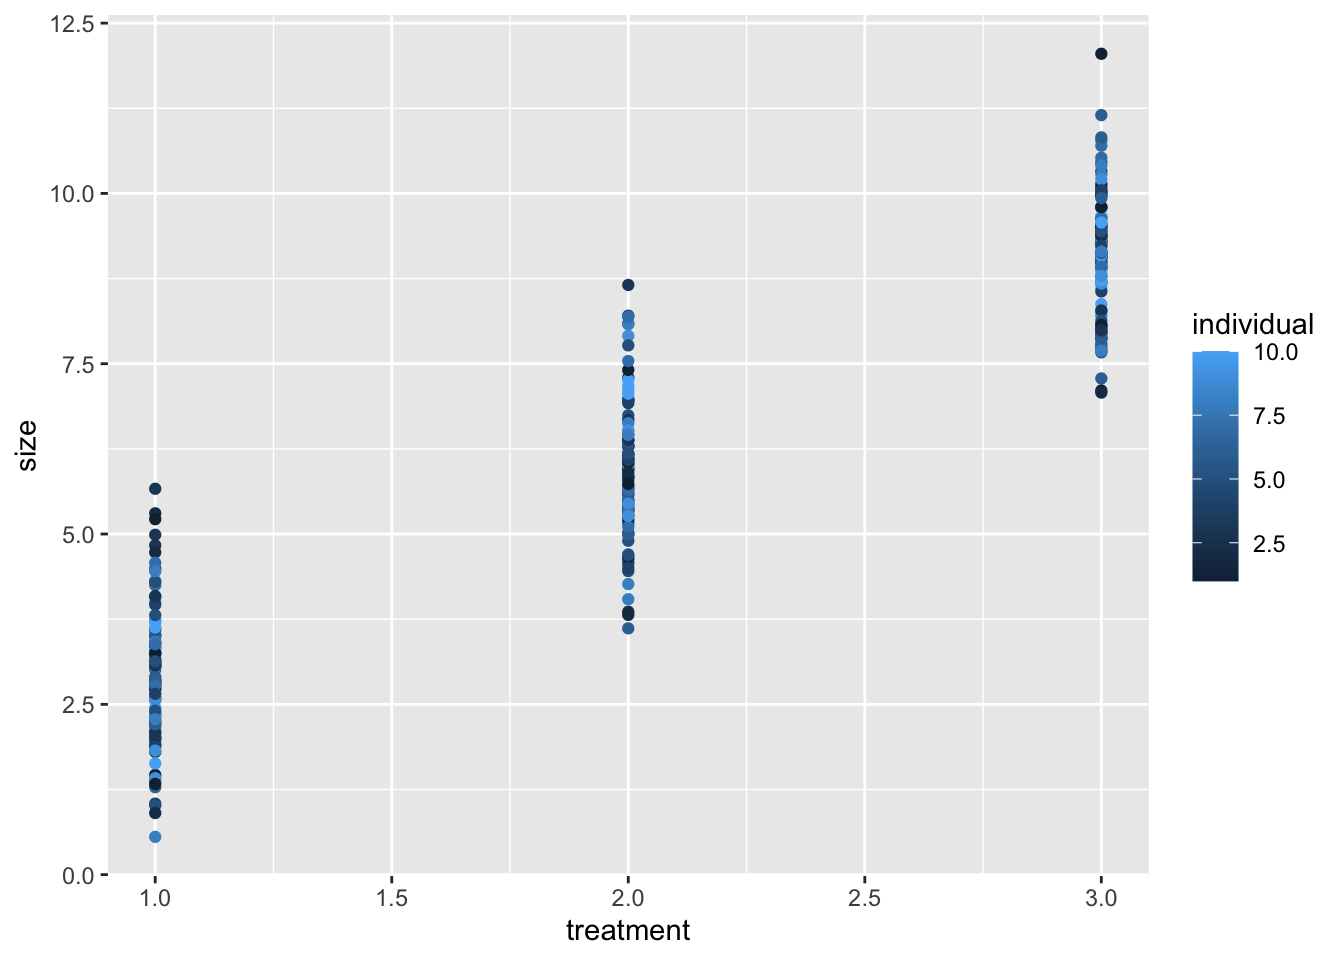
\includegraphics{03-datasets_files/figure-latex/unnamed-chunk-7-1.pdf}

\hypertarget{data-modification-conversion}{%
\section{Data modification / conversion}\label{data-modification-conversion}}

As you can see when you \texttt{print()} the contents of \texttt{super\_tbl}, all data types have the type of a \texttt{\textless{}dbl\textgreater{}} (double), which stands for double-precision floating point value. Such floating point values are typically used for data which varies in a continuous fashion, as is the case for the \texttt{size} column in \texttt{super\_tbl}.

However, we often code treatments, and sometimes also individuals (if there are only a few, like here), as discrete factors at a nominal scale, meaning that number `1' is not necessarily lower than `2', it is merely an identifier of that treatment or individual. To accomplish this, we convert the \texttt{individual} and \texttt{treatment} column from \texttt{\textless{}dbl\textgreater{}} to \texttt{\textless{}fct\textgreater{}}, which stands for factor.

To convert values into factors, we might either use the old-style function \href{https://stat.ethz.ch/R-manual/R-devel/library/base/html/factor.html}{\texttt{as.factor()}} or we might use the more modern \href{https://haven.tidyverse.org/reference/as_factor.html}{\texttt{as\_factor()}} function from the \href{https://haven.tidyverse.org/index.html}{haven} package. For this example there is no difference between both functions, but in general \texttt{as\_factor()} is slightly more generic.

How to change our data using the \texttt{as\_factor()} function? What we can do is apply the function to the columns in question, by using the \href{https://dplyr.tidyverse.org/reference/mutate.html}{\texttt{mutate()}} function from the \texttt{dplyr()} package. Using this \texttt{mutate()} function (you have been checking the examples on the manual page, right?), we can then add two new columns to our data frame, say \texttt{individual\_fac} and \texttt{treatment\_fac} which reflect our new factor data.

If we now plot our new \texttt{individual\_fac} and \texttt{treatment\_fac} columns, our plot will look slightly different:

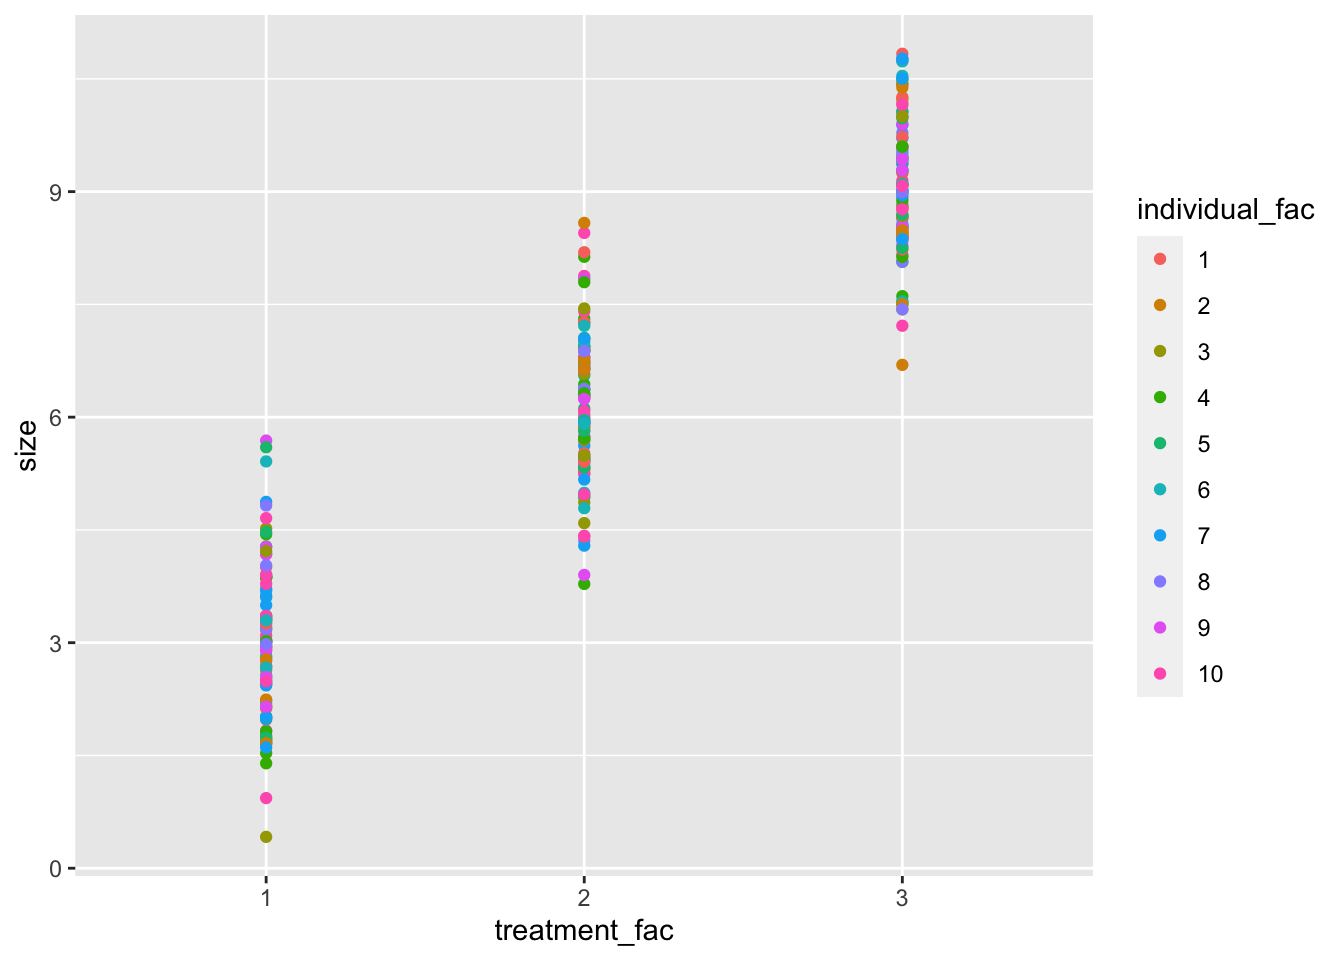
\includegraphics{03-datasets_files/figure-latex/unnamed-chunk-8-1.pdf}

Can you describe what is different between this plot and the previous one and why?

\hypertarget{a-further-aside-regular-expressions}{%
\section{A further aside: regular expressions}\label{a-further-aside-regular-expressions}}

The next exercise focuses on changing the data during the \texttt{for} loop that we used in section @ref\{forLoop\}.

Consider the following scenario: your supervisor tells you (belatedly, as always) that they have omitted some relevant detail in the previous analysis. It turns out that the size measurements in the first 4 excel sheets (i.e., \texttt{sheet\_1.xls}, \texttt{sheet\_2.xls}, \texttt{sheet\_3.xls} and \texttt{sheet\_4.xls}) were performed on a different breed of individuals (breed A), while measurements from other excel sheets used animals of breed B.

Let us visually inspect whether the relationship between treatment and size is different for the two different breeds of animals. To this end, we do not modify the underlying excel sheets, rather we add the column \texttt{breed} to the \texttt{tibble}s when reading in the data from each excel sheet. The \texttt{breed} column should have the values \texttt{A} for the first four sheets and the value \texttt{B} for the remaining sheets respectively.

A first suggestion may be to simply keep track of at which of the excel sheets we are when looping over the \texttt{xls\_sheet\_list} variable which contains all the files (see section @ref\{forLoop\}), and then set the \texttt{breed} variable according to an \texttt{if} \texttt{else} statement (i.e., first 4 files \texttt{A}, remaining files \texttt{B}). However, if you look at the listing of files in section @ref\{fileList\} above, you will see that \texttt{sheet\_10.xls} (breed \texttt{B}) is at the second position in the variable \texttt{xls\_sheet\_list}, so using a simple rule like that is not going to work.

\hypertarget{regular-expressions-to-the-rescue}{%
\subsection{Regular expressions to the rescue}\label{regular-expressions-to-the-rescue}}

Hence, we need to inspect the filenames themselves and sort out \texttt{sheet\_1.xls}, \texttt{sheet\_2.xls}, \texttt{sheet\_3.xls} and \texttt{sheet\_4.xls} from the rest. How to do this? \href{https://stat.ethz.ch/R-manual/R-patched/library/base/html/regex.html}{Regular expressions} are a great way to filter numbers from textual data.

While we are not delving into regular expressions now,

  \bibliography{refsR.bib}

\end{document}
